\documentclass{article}
\usepackage{graphicx}
\usepackage{amssymb}
\graphicspath{{./}}
\title{Altitude of a Triangle Given the Side Lengths}
\author{Michael Gionet}
\date{Nov 25th, 2023}

\begin{document}
	\maketitle
	
	\section{Theorem}
	
	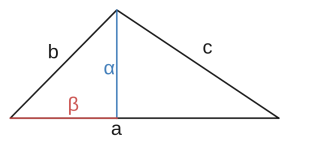
\includegraphics{altitude}
	
	
	Let $\Delta$ be the triangle with side lengths $a$, $b$, $c$. Denote the length of its altitude by $\alpha$. 
	Let $\beta$ be the length from the vertex opposite to $c$ to the altitude. Then:
	
	$$ \alpha^{2} = \frac{-(a^2 + b^2 - c^2)}{4a^{2}} + b^2 $$ 
	
	\section{Proof Outline}
	
	Since there are two right triangles in the setup, we can set up two equations using Pythagoras' Theorem. Then, we just need to isolate for $\alpha$
	
	\section{Proof}
	
	$ \square $
	
	By Pythagoras' theorem, we get the two equations:
	\begin{equation}
	b^2 = \beta^2 + \alpha^2 \label{eq:1}
	\end{equation}
	
	\begin{equation}
	c^2 = (a-\beta)^2 + \alpha^2 \label{eq:2}
	\end{equation}
	
	Subtract \ref{eq:1} from \ref{eq:2} to get:
	
	$$ b^2 - c^2 = \beta^2 - (a - \beta)^2 $$
	
	Expand:
	
	$$ b^2 - c^2 = \beta^2 - a^2 + 2 a \beta - \beta^2 $$
	
	Cancelling out term:
	
	$$ a^2 + b^2 - c^2 = 2 a \beta $$
	
	\begin{equation}
	\beta = \frac{ a^2 + b^2 - c^2 }{ 2 a } \label{eq:3}
	\end{equation}
	
	We can substitute \ref{eq:3} back into \ref{eq:1} to get:
	
	$$ b^2 = \left( \frac{ a^2 + b^2 - c^2 }{ 2 a } \right)^2 + \alpha^2 $$
	
	This gives the desired result:
	
	\begin{equation}
	\alpha^2 = \frac{ -( a^2 + b^2 - c^2 )^2 }{4 a^2} + b^2
	\end{equation}
	
	\raggedleft
	$ \blacksquare $
	
	\raggedright
	
	
	\section{A Bit of Flavor}
	
	When I was in high school, I discovered that I had a passion for mathematics at around grade 11.
	This theorem is the first one that I discovered on my own, after toying around with basic geometry. 
	
\end{document}